\documentclass[a4paper]{article}
\usepackage{amsmath}
\usepackage{amssymb}
\usepackage{amsfonts}
\usepackage{float}
\usepackage{geometry}
\usepackage{enumerate}
\usepackage{graphicx}
\usepackage{indentfirst}
\usepackage{color}
\usepackage{listings}
\usepackage{graphicx}
\usepackage{xcolor}
\usepackage{subfigure}
\usepackage[colorlinks,linkcolor=blue]{hyperref}
\usepackage{booktabs}
\usepackage{diagbox}

\setlength{\parindent}{2em}

\title{\rule[0.5cm]{\textwidth}{0.1mm}
\\KTH Royal Institute of Technology
\\\vspace{0.5em}
Machine Learning, Advanced Course
\\\vspace{0.5em}
DD2434
\\\rule[0cm]{\textwidth}{0.1mm}\vspace{4em}}

\author
{\Large\textbf{{Project -- Large Network representation learning}}
\\\\\\\\\\\vspace{0.5em}
\Large{\textbf{Group 2}}\\\vspace{0.2em}
\Large{Jiaming Huang}\\\vspace{0.2em}
\Large{Tianzhang Cai}\\\vspace{0.2em}
\Large{Wenhao Luo}\\\vspace{0.2em}
\Large{Zhengjie Ji}
\\\vspace{2em}}

\newcommand{\citehere}{\textcolor[rgb]{1,0,0}{CITE\ }}
\newcommand{\noun}[1]{\textsc{#1}}
\newcommand{\tabincell}[2]{\begin{tabular}{@{}#1@{}}#2\end{tabular}}  

% ================
\usepackage[style = ieee, urldate =comp]{biblatex}
\addbibresource{bib.bib}
% ================

\begin{document}

\maketitle
\thispagestyle{empty}



\vspace{1em}\noindent \textbf{Abstract} We reproduce the empirical study on unsupervised network representation learning (UNRL) approaches over graphs, considering 5 UNRL techniques and two common tasks – node classification and link prediction. We found that ?(Ex:  We find that for non-attributed graphs there is no single method that is a clear winner and that the choice of a suitable method is dictated by certain properties of the embedding methods, task and structural properties of the underlying graph. In addition we also report the common pitfalls in evaluation of UNRL methods and come up with suggestions for experimental design and interpretation of results.)
% Abstract: overview of this project

\newpage
\setcounter{page}{1}

% title, group number, author list, and short abstract

\section{Introduction}
% Introduction: what the original paper did, what we are going to do in general

%In the report, you should first in the Introduction describe the article in such a level of detail that your peer students in this course understand the method, and so that it is clear to the reader that you understand the method too. You can put it in a wider context of the more recent state-of-the-art work that is built on the original contribution. Towards the end of the introduction, you should clearly and concisely outline the scope and objectives of your project.

% why need to do comparison? 
% key findings in the paper
% what we de in this project



\noindent In this project we reproduce the results of the article “A Comparative Study for Unsupervised Network Representation Learning \cite{1}” according to the requirements of the assignment. The original article conducted a large-scale study on multiple unsupervised network representation learning algorithms, and made a systematic comparison on their performance in different tasks. We implemented five methods mentioned in the article: DeepWalk, Node2vec, Line, NetMF and GraphSage, and apply them to two tasks: node classification and link prediction, evaluating on different datasets. Based on our results, we verify and further explore the research results of the article.


\subsection{Study Background}

% framework

\noindent To understand how various methods differ in definitions and treatment of similarity, we introduce the concept of context graph. A context graph is defined as a graph with the weight of edge (u,v) denote the similarity between u and v, where negative weight means dissimilarity between the two nodes. And the representation of a node is divided into “source” and “context”. The source role of node v is obtained by the observable edges, and the context of v is its “one-hop neighbor” \cite{1}. We would like to use different methods to learn and analyze the source and context representation of nodes.


\subsection{Research Questions} 


\noindent In our experiment, we hope to answer the following research questions. These questions are adapted from that asked in the original paper \citehere.

\begin{enumerate}[1.]

\item How does the choice of different methods affect the performance of assigned tasks?

\item How does the choice of different ways of exploiting the context affect the performance of network representation learning methods? 

\item How does the choice of optimization method affect the performance? Do deep models always outperform the shallow models? 

\item Do these methods have good generalization ability to new datasets?

\end{enumerate}

\section{Procedure}
% How we conduct the experiment, step by step

\noindent The procedure of our experiment are as follows, according to the requirements of the project assignment.

\begin{enumerate}[1.]

\item Implement five methods discussed in the paper: DeepWalk, Node2vec, Line-1, NetMF, and GraphSage. 

\item Collect all the datasets presented in the paper and a few additional datasets.

\item Evaluate the different methods on the data we collected with respect to the tasks of link prediction and node classification.

\item Discuss our findings and give answer to the research questions we posted based on our results.

\item Compare our results to the results of the paper, and discuss the reproducibility of the study.

\item Discuss the original paper in terms of approach, methodology, and conclusions.

\end{enumerate}


\section{Methods}

%You should then present your re-implementation or extension of the method in the Methods section, and your reproduction of the results in the Results section. Again, please communicate on such a level that your peer students understand what you have done, and so that it is clear to the reader what results you got and if, how, and why they deviate from the results presented in the original article. Alternatively, if you extended or modified the original method please state clearly the motivation and your reasoning behind it, and describe how your results relate to those in the original paper.

\noindent In this part, we introduced the principle of the algorithms that we re-implemented and our extensions of these methods.


% Methods: Algorithm Description, Task Description. Each algorithm/task includes: 1. how it works, 2. our re-implementation, 3. our extension

\subsection{Algorithm Description}
% For each algorithm, we need to write: the algorithm itself, the optimization
\noindent In this part, we introduce the five unsupervised embedding methods analyzed in this project, DeepWalk, Node2vec, Line, NetMF and GraphSage.

\begin{table}[H]
\centering
\begin{tabular}{|c|c|c|c|}
\hline
method & \tabincell{c}{Formulation of \\ Context Graph} & Learned Embeddings & Optimization Methods\\
\hline
DeepWalk& \tabincell{c}{Random Walk}&  Source and Context &\tabincell{c}{Hierarchical Softmax}\\
\hline
Node2vec& \tabincell{c}{Random Walk}&  Source and Context &\tabincell{c}{Negative Sampling}\\
\hline
LINE-1& \tabincell{c}{Adjacency Based} &  Source &\tabincell{c}{Negative Sampling}\\
\hline
NetMF& \tabincell{c}{Context Matrix} & Source and Context& \tabincell{c}{Context Matrix Factorization} \\
\hline
GraphSage&  \tabincell{c}{Random Walk} & Source&\tabincell{c}{Neighborhood Aggregation \\ and Negative Sampling} \\
\hline
\end{tabular}
\caption{Comparison of methods in terms of schemes of defining context, exploitation of context and optimization methods.}
\end{table}


\subsubsection{Random Walk Based Methods} %deepwalk, node2vec

\noindent \textbf{DeepWalk} utilizes random walk to sample a sequence of graph nodes where for each node, its successive node is randomly selected from its neighbors. After the random walk sequence is sampled, a window of a certain width slides through it and at each position, the node at the window center forms a \emph{context edge} with each of the rest nodes in the window. For these context edges $C$, we want to find the graph embeddings $\Phi$ and $\theta$ such that the loss 
$$
-\sum_{(u,v)\in C}\log P(v\mid u)=-\sum_{(u,v)\in C}\log\frac{\exp(\Phi_u\cdot \theta_v)}{\sum_{w\in V}{\exp(\Phi_u\cdot \theta_w)}},
$$
is minimized, which is equivalent to maximizing the likelihood of the co-occurrence of nodes in the same context. However, note that in the denominator there is a sum over all nodes in the graph, which makes the objective function computationally very expensive. To deal with this, two methods have been proposed: hierarchical SoftMax and negative sampling. In the original paper, DeepWalk adopts hierarchical SoftMax, which constructs a Huffman binary tree in which each graph node is a leaf \citehere{}. In this manner, the log probability is approximated by traversing the tree bottom up, thus reducing the time complexity to $O(\log V)$. After the loss is obtained, we use back-propagation and gradient descent to optimize the graph embeddings. \\  

\noindent \textbf{Node2Vec} The major difference between DeepWalk and Node2Vec is the probability distribution of the neighborhood selection. For DeepWalk, the distribution is uniform - each neighbor is equally likely to be selected. For Node2Vec, the distribution of neighbors is dependent on the list of nodes in the random walk - more specifically, dependent on the node preceding the current node in the walk, which is called the second-order neighborhood \citehere{}. Intuitively, the probability distribution of the second-order neighborhood in Node2Vec is controlled by 2 parameters $p$ and $q$ - they control the probabilities of the next node coming back or walking away from the previous one respectively. Hence, Node2Vec is actually a generalization of DeepWalk. When $p = q = 1$, the neighborhood distribution in Node2Vec is unbiased and thus the same as that in DeepWalk.

\subsubsection{Adjacency Based Methods} % Line, GraphSAGE

\noindent \textbf{LINE} \citehere aims to preserve both local and global network structures in embedding. "First order proximity" is captured by observable links between vertic es. And "Second order proximity" is determined through the neighbors shared between vertices. LINE-1 optimizes the "First order proximity", which preserves the local network structure, and LINE-2 deal with the "Second order proximity" and global structure. The optimization is done by stochastic gradient descent. To improve the efficiency and to avoid a huge weight multiplying to the gradients, LINE samples the edges with probability proportional to their weights.


\subsubsection{Matrix Factorization Based Methods} % NetMF


\noindent \textbf{NetMF} This method unified LINE, PTE, DeepWalk and Node2vec in the framewalk of matrix factorization. It directly factorizes the context matrix with $(i,j)$th element given by \citehere:
$$
c_{i,j} = log(\frac{vol(G)}{kT}(\frac{1}{d_j} \cdot (\sum\limits_{r=1}^T P^r)_{i,j}))
$$
\noindent where $T$ is the window size, $r$ is the walk length and $k$ is the number of negative samples in DeepWalk. For small window size $T$, we first compute the DeepWalk matrix $M$, and then factorize (perform SVD) to get the network embedding. For large window size $T$, it is not feasible to directly compute the DeepWalk matrix $M$ as the time complexity can be too high. A solution to this is to approximate the DeepWalk matrix $M$ and show its low-rank nature by using the relationship of  $M$ with the normalized graph Laplacian.

\subsubsection{Neural Network Based Methods} % GraphSage
GraphSage is a framework of graph neural network that leverages neighborhood aggregation to inductively learn the topological structure of each node's neighborhood and incorporate them into the node embeddings. A variety of \emph{aggregator functions} can be used in the GraphSage framework. The simplest one is the \textit{mean} function, which aggregates the neighborhood information by taking the mean of the embedding of each neighbor. 

\subsection{Task Description}

\noindent In this part, we describe the two tasks that we used for comparing the Unsupervised Network Representation Learning (UNRL) methods.

\subsubsection{Link Prediction (LP)}

\noindent The first task is to predict missing edges of a network. In the original paper describing the experiments of Link Prediction \citehere, the author work with the subgraphs of a social network $G$ with potentially different time-stamps. In this article \citehere, we instead evaluate a network with a fraction of removed edges (no vertex is isolated due to the removal). The residual network is used for training, and the removed edges are served as the test split. Also, we sample negative edges to balance the test split. In the training process, we measure the distance (similarity) between pair of vertices using four different methods: common neighbors, Jaccard's coefficient, Adamic/Adar and preferential attachment. Then we rank the node-to-node similarity and predict links according to the rank. To obtain the accuracy of the prediction, we test our prediction on the test split and calculate the ROC-AUC (Area Under the Receiver Operating Characteristic Curve) scores.

\subsubsection{Multilabel Node Classification (NC)}

\noindent The second task is to do node classification on a graph where each node has one or more labels. We do the multilabel classification using one-vs-rest logistic regression. Then, we test the accuracy using 5-fold cross validation, and report the mean Micro-F1 and Macro-F1 scores.


\section{Implementation}

\subsection{Datasets}
\noindent In this part, we introduce the datasets used in our experiment for different tasks. For the Reddit, Youtube and Twitter, due to the limitation of computation resources, it is difficult for us to conduct experiment on these extreme large datasets, so we are unable to present results on them. For node classification, we test the different algorithms on BlogCatalog, Cora, Pubmed, Cocit, Flickr. For link prediction, Blogcatalog, Flikcr, Cora, DBLP-Ci and Epinion were used. The detail of these datasets are summarized in table 2.
\begin{table}[H]
    \centering
\begin{tabular}{c|c|c|c|c|c|c}
\toprule  
& BlogCatalog& Cora & Pubmed& Cocit &DBLP-Ci &Epinion\\
\midrule  
Category & SN& Citation&Citation&Citation&Citation &SN\\
Type& undir& dir & dir & dir & dir & dir\\
$|V|$ &10k &2.7k &19k &44k &12.5k & 75k\\
$|E|$ &333k & 5.4k &44k & 195k &49k &508k\\
\bottomrule 
\end{tabular}
\caption{Summary of datasets used in our experiment. SN denotes social networks.}
\end{table}





\subsection{Parameter settings}
\noindent Most of the parameters are the same as the parameters in \cite{1}. Part of them are modified due to some special reasons.
\begin{table}[H]
    \centering
\begin{tabular}{c|c|c|c}
\toprule  
Parameter& Value& Parameter &Value\\
\midrule  
Embedding dimension d & 128& Walk length t&40\\
Number of Walk r& 80& Window size w& 10\\
Negative Sample Size ns & 5& LINE iteration& 300000\\
Number of Eigenpairs h & 256& NODE2VEC p,q& 0.25,4\\
\bottomrule 
\end{tabular}
\caption{Parameters we used and the corresponding values.}
\end{table}
\noindent The iteration number for LINE is reduced from 10 billion to 300000, mainly because it is too time-consuming and we cannot get a result in time by our hardware.



\subsection{Hardware and Software}

\section{Results}

\noindent In this part, we demonstrate the results that we obtained applying each method to the two tasks discussed above. 


%
%\begin{figure}[H]
%\centering  
%\subfigure[Plot for real graph "example1.dat"]{
%\label{Fig.sub.1}
%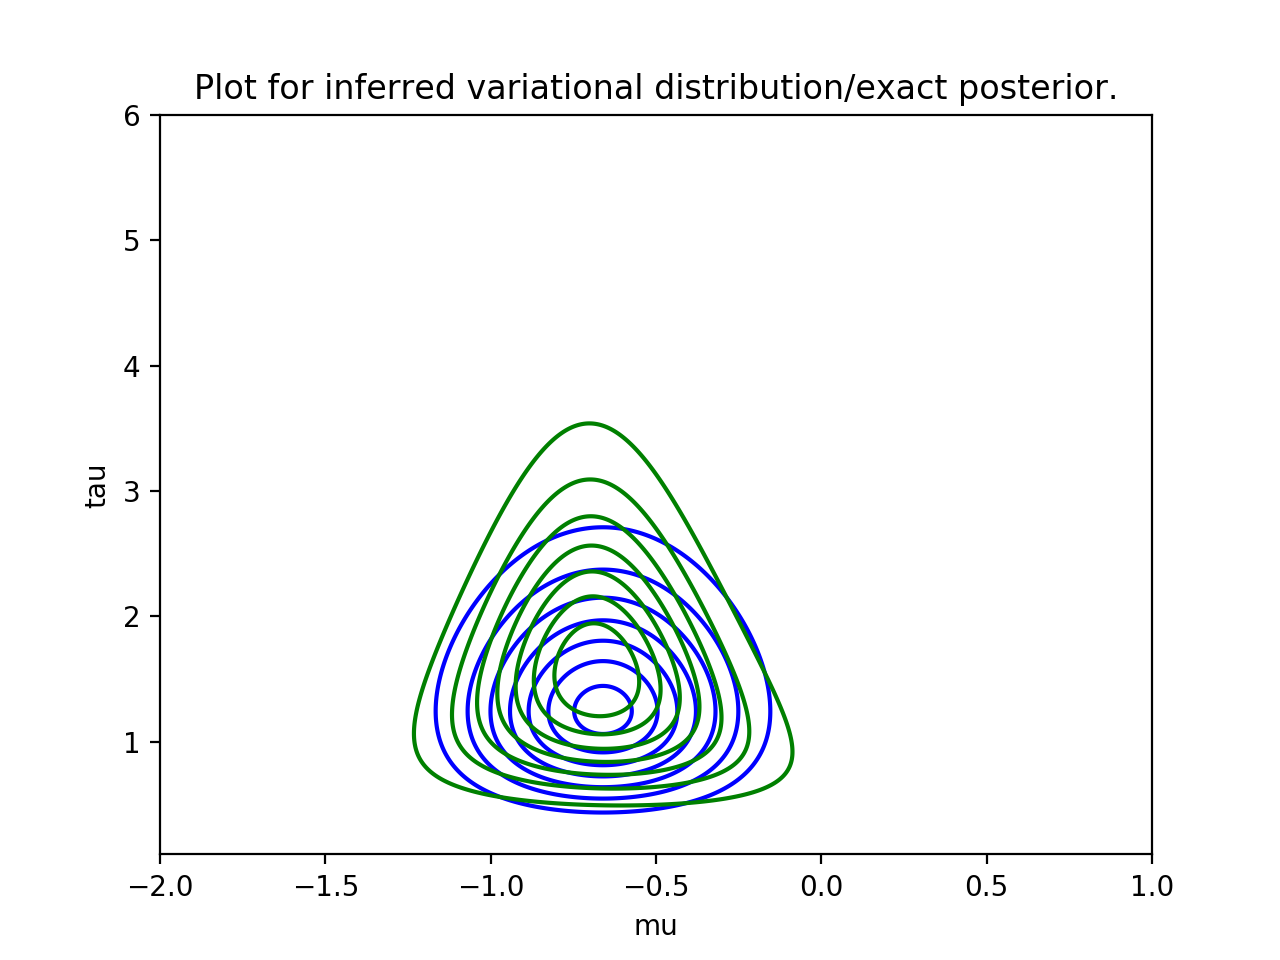
\includegraphics[width=0.45\textwidth, height=0.27\textwidth]{sample.png}}
%\subfigure[Plot for synthetic graph "example2.dat"]{
%\label{Fig.sub.2}
%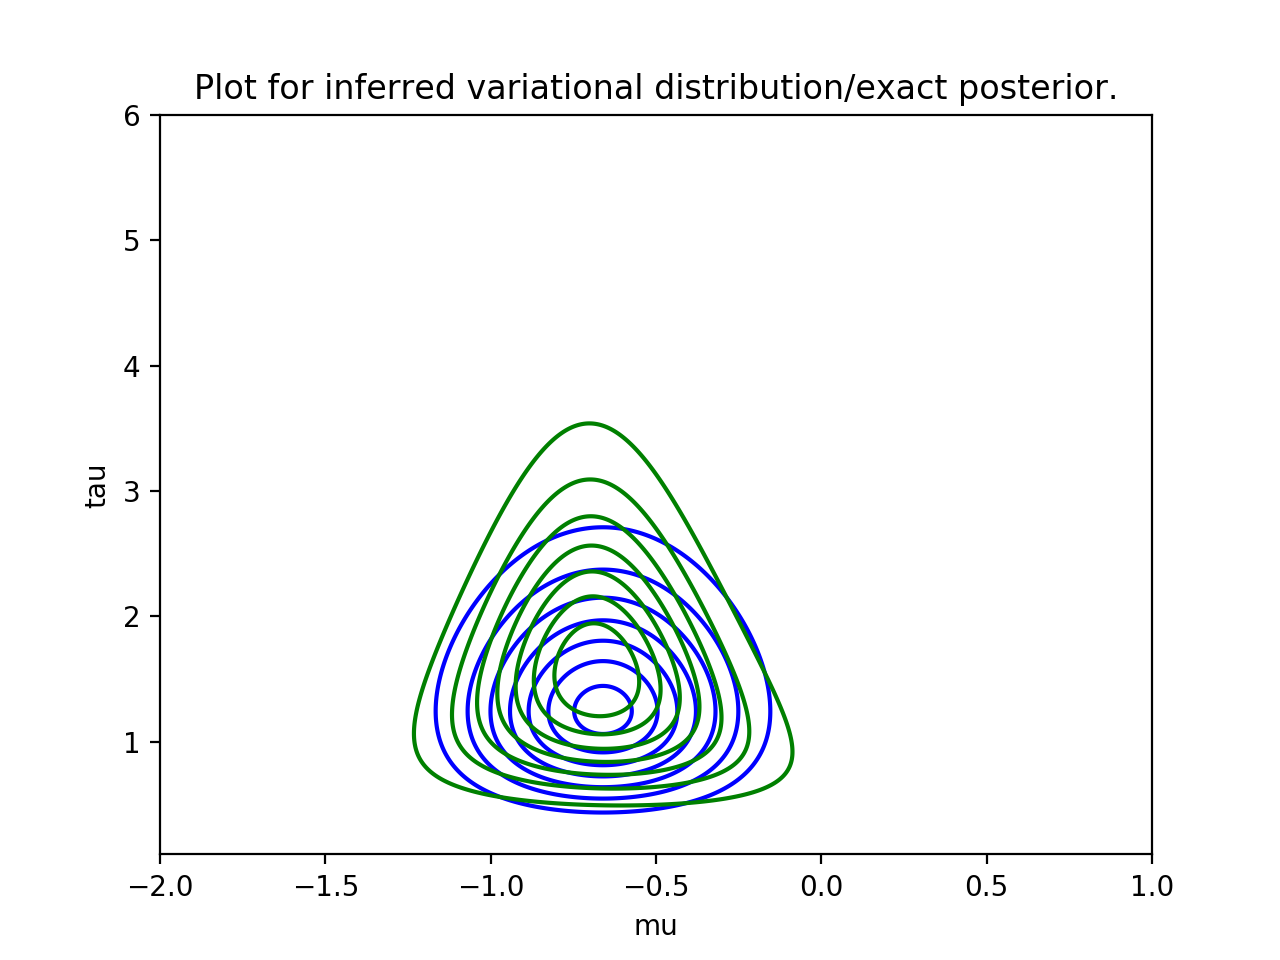
\includegraphics[width=0.45\textwidth, height=0.27\textwidth]{sample.png}}
%\caption{Plots of adjacency matrix.}
%\label{Fig.main}
%\end{figure}

\subsection{Link Prediction (LP)}

% accuracy
% convergence speed

\noindent Here we demonstrate the result for link prediction. We evaluate the five methods mentioned above on four datasets: BlogCatalog, Cora, Lesmis (additional) and Facebook (additional).

\begin{table}[H]
\centering
\begin{tabular}{|c|c|c|c|c|c|}
\hline
method & BlogCatalog & Cora & PubMed & Lesmis & Facebook\\
\hline
DeepWalk& \textcolor{red}{0.000}& \textcolor{red}{0.000}& \textcolor{red}{0.000}& \textcolor{red}{0.000}& \textcolor{red}{0.000}\\
Node2vec& \textcolor{red}{0.000}& \textcolor{red}{0.000}& \textcolor{red}{0.000}& \textcolor{red}{0.000}& \textcolor{red}{0.000}\\
LINE-1& \textcolor{red}{0.000}& \textcolor{red}{0.000}& \textcolor{red}{0.000}& \textcolor{red}{0.000}& \textcolor{red}{0.000}\\
NetMF& \textcolor{red}{0.000}& \textcolor{red}{0.000}& \textcolor{red}{0.000}& \textcolor{red}{0.000}& \textcolor{red}{0.000}\\
GraphSage& \textcolor{red}{0.000}& \textcolor{red}{0.000}& \textcolor{red}{0.000}& \textcolor{red}{0.000}& \textcolor{red}{0.000}\\
\hline
\end{tabular}
\caption{Link Prediction results using 50\% edges as training data, balanced with negative edges. Blue indicates that our results are better than the original paper, and vice versa.}
\end{table}


\subsection{Multilabel Node Classification (NC)}

\noindent Here we demonstrate the result for Multilabel Node Classification. We evaluate the five methods mentioned above on three datasets: BlogCatalog, Cora, PubMed and Chameleon (additional). In most cases we achieved lower scores than that of the original paper. blablabla

\begin{table}[H]
\centering
\begin{tabular}{|c|c|c|c|c|c|c|c|c|}
\hline
method & \multicolumn{2}{|c|}{BlogCatalog}& \multicolumn{2}{|c|}{Cora}& \multicolumn{2}{|c|}{PubMed} & \multicolumn{2}{|c|}{Chameleon}\\
\hline
& mic. & mac. &mic. & mac.& mic. & mac.& mic. & mac.\\
\hline
DeepWalk& \textcolor{red}{\textbf{0.336}}& \textcolor{red}{\textbf{0.195}}&\textcolor{red}{0.000}&\textcolor{red}{0.000}&\textcolor{red}{0.645}&\textcolor{red}{0.548}&\textcolor{red}{0.000}&\textcolor{red}{0.000}\\
Node2vec& \textcolor{red}{0.192}& \textcolor{red}{0.088}&\textcolor{red}{0.000}&\textcolor{red}{0.000}&\textcolor{red}{0.603}&\textcolor{red}{0.558}&\textcolor{red}{0.000}&\textcolor{red}{0.000}\\
LINE-1& \textcolor{red}{0.161}& \textcolor{red}{0.064}&\textcolor{red}{0.000}&\textcolor{red}{0.000}&\textcolor{red}{0.345}&\textcolor{red}{0.271}&\textcolor{red}{0.000}&\textcolor{red}{0.000}\\
NetMF& \textcolor{red}{0.191}& \textcolor{red}{0.091}&\textcolor{red}{0.000}&\textcolor{red}{0.000}& \textcolor{cyan}{\textbf{0.808}}&\textcolor{cyan}{\textbf{0.794}}&\textcolor{red}{0.000}&\textcolor{red}{0.000}\\
GraphSage& \textcolor{red}{0.000}& \textcolor{red}{0.000}&\textcolor{red}{0.000}&\textcolor{red}{0.000}&\textcolor{red}{0.000}&\textcolor{red}{0.000}&\textcolor{red}{0.000}&\textcolor{red}{0.000}\\
\hline
\end{tabular}
\caption{Multilabel Node Classification results in terms of Micro-F1 and Macro-F1. All results are mean of 5-fold cross validations. Blue indicates that our results are better than the original paper, and vice versa.}
\end{table}


\section{Discussion}

%Finally, you should critically discuss the methods and findings included in your report. Please, argue in favor and against the method in relation to the authors' arguments and their line of reasoning. In this Discussion section please provide a wider context potentially taking into account more recent developments built on the original contributions made in the paper (or as a countermeasure to these original contributions).

\subsection{Discussion of Our Findings}

\noindent In this part, we discuss our findings and give answer to the research questions in the Introduction section based on our results.\\

\noindent Inspect into our result, we can see that blabla \\

\noindent Now, we give answer to the research questions.
\begin{enumerate}[1.]
\item How does the choice of different methods affect the performance of assigned tasks? \\
\textbf{Answer}: blabla

\item How does the choice of different ways of exploiting the context affect the performance of network representation learning methods?\\
\textbf{Answer}: blabla

\item How does the choice of optimization method affect the performance? Do deep models always outperform the shallow models?\\
\textbf{Answer}: blabla

\item Do these methods have good generalization ability to new datasets?\\
\textbf{Answer}: blabla

\end{enumerate}

\subsection{Comparison of Results}
% Compare our results to the results of the paper, and discuss the reproducibility of the study.


\subsection{Discussion about the Original Paper}

% Discuss the original paper in terms of approach, methodology, and conclusion


\section{Conclusions}

\noindent Here we write something. 



\newpage
% ================
\printbibliography
% ================

\end{document}

